\section{Theory}

Magnetic resonance is a quantum phenomenon that describes the resonant interaction between spins and electromagnetic fields. It has significant applications in fields such as medicine, science, and technology. Magnetic resonance imaging (MRI) is an indispensable non-invasive technique used in medical diagnosis and research. Nuclear magnetic resonance (NMR) spectroscopy is widely employed in physics, chemistry, biology, and materials science for examining the physical and chemical properties of substances, as well as for identifying their distinct characteristics.

When a magnetic needle with a magnetic moment
$\vec{m}$ is placed in a magnetic field composed of a strong permanent magnet $\vec{B}_{PM}$ and the Earth's magnetic
field $\vec{B}_E$, the torque acting on the needle is given by,

\begin{align}
    \vec{T} = \Vec{m} \cross (\vec{B}_{PM}+\vec{B}_E)
\end{align}

However, since the magnetic field of the permanent magnet is much stronger than that of the Earth's magnetic field, $\vec{B}_E$ can be neglected. Therefore, the torque simplifies to

\begin{align}
    \vec{T} = \Vec{m} \cross \vec{B}_{PM}
\end{align}

Now, consider an alternating magnetic field $\vec{B}_\text{drive}$ produced by a coil with alternating current. This drive field will cause the magnetic needle to oscillate in the horizontal plane (the compass plane). Since the permanent magnet is aligned along the x-axis, the sum of the torques due to the permanent magnet and the coil's field is equal to the time-derivative of the angular momentum of the needle,

\begin{align}
    \Vec{m} \cross (\vec{B}_{PM} +\vec{B}_\text{drive}) = J\frac{d\theta}{dt}\hat{z} 
\end{align}

where $J$ is the moment of inertia of the needle, and $\theta$ is the deflection angle.
For small angles, we can approximate $\sin\theta \approx \theta$ and $\sin(\pi/2 - \theta) \approx 1$. Substituting these into the z-component of the torque equation,

\begin{align}
    mB_{PM}\sin \theta + mB_\text{drive}\sin(\frac{\pi}{2} - \theta) &= J\frac{d\theta}{dt}\\
    \implies mB_{PM}\theta + mB_\text{drive} &= J\frac{d^2\theta}{dt^2}
\end{align}

This is a differential equation for a driven harmonic oscillator. The equation can be written as

\begin{align}
    \frac{d^2\theta}{dt^2}+\omega_0^2\theta=\omega^2
\end{align}

where,

\begin{align}
    \omega_0 = \sqrt{\frac{mB_{PM}}{J}} \text{  and  } \omega = \sqrt{\frac{mB_\text{drive}}{J}}
\end{align}

This equation describes a harmonic oscillator wit a natural frequency $\omega_0$. When the driving frequency $\omega$  matches the natural frequency $\omega_0$, resonance occurs, leading to a significant increase in the oscillation amplitude.

In the experiment, the frequency of the coil's alternating current is kept constant. By adjusting the distance $d$ between the permanent magnet and the
compass, the magnetic field $\vec{B}_{PM}$ experienced by the compass changes. The magnetic field of the permanent magnet at a distance $d$ is given by the dipole approximation

\begin{align}
    B_{PM} = \frac{\mu_0}{4\pi}\frac{2m_{PM}}{d^3}
\end{align}

where $m_{PM}$ is the magnetic moment of the permanent magnet. The resonance frequency is then

\begin{align}
    f_\text{res} = \frac{1}{2\pi}\sqrt{\frac{\mu_0}{4\pi}\frac{m_{PM}}{d^3}\frac{m}{J}}
\end{align}

This formula shows how the resonance frequency depends on the distance between the permanent magnet and the compass as well as on the magnetic
moment of the permanent magnet. The final working formula is given by

\begin{align}
    f_\text{res} = \frac{1}{2\pi}\sqrt{B_{PM}\frac{m}{J}}
\end{align}

% ==========================================================================
\section{Experimental Setup}

\subsection*{Apparatus}

\begin{enumerate}
    \item Neodymium magnet
    \item Function Generator
    \item Circular Coiled wire
    \item Platform with distance label
    \item Compass\\
\end{enumerate}

When we place a compass on a table, the needle naturally aligns with the Earth's magnetic field. If we then introduce a much stronger permanent magnet near the compass, the needle will realign itself towards the magnet. A similar effect occurs if we position the compass near an electromagnetic coil carrying a constant current.

\begin{figure}[H]
    \centering
    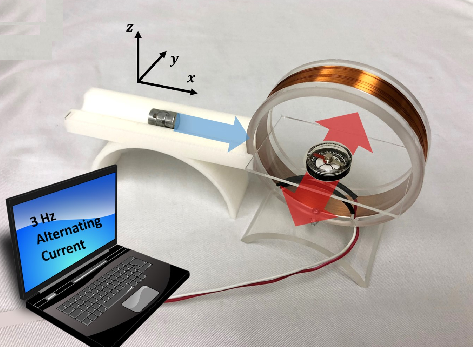
\includegraphics[width=1\columnwidth]{images/f.png}
    \caption{Schematic Diagram of the setup}
\end{figure}

However, if we instead pass a weak alternating current through the coil, the needle won't fully follow the alternating magnetic field. Instead, it will oscillate around its initial alignment with the permanent magnet when both the permanent magnet and the electromagnetic coil are present. The oscillation of the needle remains minimal when the permanent magnet is either too close or too far from the compass. However, at an intermediate distance between the compass and the permanent magnet, the oscillations become significantly stronger, indicating resonance.